\documentclass[11pt]{article}
\usepackage[paperwidth=254mm,paperheight=142.875mm,margin=12mm]{geometry}
\usepackage{amsmath,amssymb,mathtools}
\usepackage{newtxtext,newtxmath}  % TIMES: HEAVIER STROKES THAN COMPUTER MODERN, READS BETTER ON A TINTED BLOCK
\usepackage{graphicx}
\usepackage{booktabs}
\usepackage{xcolor}
\definecolor{blockbg}{RGB}{240,245,252}
\definecolor{blockrule}{RGB}{140,165,200}
\definecolor{accent}{RGB}{22,54,110}
\usepackage[hidelinks]{hyperref}
\usepackage{tikz}
\usetikzlibrary{positioning,arrows.meta,fit,calc}
\tikzset{
  fl/.style={draw=gray!70,fill=white,rounded corners=2pt,minimum height=12mm,minimum width=15mm,align=center},
  ql/.style={fl,draw=blue!60!black,fill=blue!12,very thick},
  arr/.style={-{Stealth[length=2mm]},thick},
}

\newcommand{\R}{\mathbb{R}}
\newcommand{\Var}{\operatorname{Var}}
\newcommand{\Cov}{\operatorname{Cov}}
\newcommand{\point}[2]{\item \textbf{#1}\par\vspace{3pt}{\centering #2\par}}
\newcommand{\plainpoint}[2]{\textbf{#1}\par\vspace{7pt}{\centering #2\par}\vspace{18pt}}
\newcommand{\hl}[1]{{\setlength{\fboxsep}{2pt}\colorbox{yellow!45}{$\displaystyle #1$}}}
\newsavebox{\blockbox}
\newenvironment{shadedblock}[1][]
  {\par\vspace{8pt}\setlength{\fboxsep}{8pt}\setlength{\fboxrule}{0.6pt}%
   \begin{lrbox}{\blockbox}\if\relax\detokenize{#1}\relax
   \begin{minipage}{\dimexpr\linewidth-2\fboxsep-2\fboxrule\relax}\else
   \begin{minipage}[t][#1]{\dimexpr\linewidth-2\fboxsep-2\fboxrule\relax}\vspace{0pt}\fi}
  {\end{minipage}\end{lrbox}\noindent\fcolorbox{blockrule}{blockbg}{\usebox{\blockbox}}\par}

\newcommand{\slide}[1]{\clearpage\noindent{\Large\bfseries\color{accent}#1}\par\vspace{4pt}{\color{accent}\hrule}\vspace{10pt}}

\begin{document}

% TITLE SLIDE
\clearpage
\vspace*{\fill}
\begin{center}
{\LARGE\bfseries Robust Training of Neural Networks\\[4pt] at Arbitrary Precision and Sparsity}\par\vspace{8pt}
{\large C.~Ye, G.~Chu, Y.~Liu, Y.~Zhang, L.~Lew, L.~Zhang, M.~Sandler, A.~Howard}\par
{\large Google DeepMind \quad\textbullet\quad ICLR 2026}\par\vspace{28pt}
{\large Presented by}\par\vspace{6pt}
{\Large Ayush Srivastava (2026AIB2015)\qquad Sarvesh Nikas (2026AIB2045)}
\end{center}
\vspace*{\fill}

\slide{Why quantization, and the forward pass during training}

\newcommand{\introheight}{30mm}
\noindent
\begin{minipage}[t]{0.40\textwidth}
\begin{shadedblock}[\introheight]
\textbf{Why quantization.}
\begin{itemize}\setlength{\itemsep}{4pt}
\item Billions of weights, each 32 or 16 bits.
\item Too big for a phone, slow, costly in energy.
\item Quantization: 4, 2 or 1 bit per weight.
\end{itemize}
\end{shadedblock}
\end{minipage}\hfill
\begin{minipage}[t]{0.58\textwidth}
\begin{shadedblock}[\introheight]
\textbf{Training with quantization.}
\begin{itemize}\setlength{\itemsep}{4pt}
\item Training keeps the float weights $x$.
\item Forward pass uses quantized $\hat x$; backward pass updates the float $x$.
\item Inference keeps only $\hat x$ (stored as $q$ plus $s_f$, $b_f$ per block).
\end{itemize}
\end{shadedblock}
\end{minipage}

\begin{shadedblock}
\paragraph{The forward pass during training.}
\[
x\ \xrightarrow{\ f\ }\ f(x)\ \xrightarrow{\ \operatorname{round}\ }\ q\ \xrightarrow{\ s_f q+b_f\mathbf 1\ }\ \hat x\ \longrightarrow\ \text{rest of network}\ \longrightarrow\ L
\]
\begin{itemize}
\item $x\in\R^N$: float block, kept and updated during training.
\item $f(x)=\dfrac{x-b_f\mathbf 1}{s_f}$: rescales $x$ onto the $k$-bit integer grid $\{0,\dots,2^k-1\}$, with $s_f=\dfrac{x_{\max}-x_{\min}}{2^k-1}$, $b_f=x_{\min}$.
\item $q=\operatorname{round}\big(f(x)\big)=f(x)+\delta$: the integers, with rounding error $|\delta_i|\le\frac12$.
\item $\hat x=s_f\,q+b_f\mathbf 1=x+s_f\,\delta$: $x$ as seen after quantization; this is what the next layer uses.
\end{itemize}
\end{shadedblock}

\slide{What gets quantized, and where}
\newcommand{\qrows}[2]{%
\node[lb] (x) at (0,0) {activations $x$\\[-1pt]\footnotesize one block per token};
\node[lb] (w) at (0,-17mm) {weights $W$\\[-1pt]\footnotesize #1};
\node[ql] (qx) at (44mm,0) {scale, round\\$q_X$};
\node[ql] (qw) at (44mm,-17mm) {#2};
\draw[arr] (x) -- (qx); \draw[arr] (w) -- (qw);}

\vspace{6pt}
\noindent\textbf{Training time.}\quad Rebuild in float, so gradients can flow.
\begin{shadedblock}
\centering
\begin{tikzpicture}[lb/.style={fl,text width=36mm},rb/.style={fl,text width=30mm}]
\qrows{one block per row}{scale, round\\$q_W$}
\node[rb] (rx) at (84mm,0) {rebuild\\$\hat x$ \ or \ $g(q_X)$};
\node[rb] (rw) at (84mm,-17mm) {rebuild\\$\hat W$ \ or \ $g(q_W)$};
\node[fl] (mm) at (122mm,-8.5mm) {float\\matmul};
\node (y) at (140mm,-8.5mm) {$y$};
\foreach \a/\b in {qx/rx,qw/rw,mm/y} \draw[arr] (\a) -- (\b);
\draw[arr] (rx.east) -- (mm.north west);
\draw[arr] (rw.east) -- (mm.south west);
\node[anchor=west,align=left] at (150mm,-8.5mm) {\textbf{STE:} $\hat x=s_f\,q+b_f\mathbf 1$.\\[4pt]\textbf{With $g$:} fitted $s_g,\,b_g$.\\[4pt]\textbf{Backward:} updates float $W$.};
\end{tikzpicture}
\end{shadedblock}

\vspace{16pt}
\noindent\textbf{Inference time.}\quad Multiply integers only; apply scales afterwards.
\begin{shadedblock}
\centering
\begin{tikzpicture}[lb/.style={fl,text width=36mm},rb/.style={fl,text width=30mm}]
\qrows{float copy dropped}{stored $q_W$\\[-1pt]\footnotesize plus $s_g,b_g$ per row}
\node[ql,text width=30mm] (mm) at (84mm,-8.5mm) {integer matmul\\$q_X\,q_W$};
\node[fl] (rs) at (122mm,-8.5mm) {rescale,\\shift};
\node (y) at (140mm,-8.5mm) {$y$};
\draw[arr] (qx.east) -- (mm.north west);
\draw[arr] (qw.east) -- (mm.south west);
\foreach \a/\b in {mm/rs,rs/y} \draw[arr] (\a) -- (\b);
\node[anchor=west,align=left] at (150mm,-8.5mm) {\textbf{Weights:} $s_g,b_g$ precomputed.\\[4pt]\textbf{Activations:} $s_g,b_g$ per token.};
\end{tikzpicture}
\end{shadedblock}

\slide{The problem: the true gradient is zero}

\begin{shadedblock}
\paragraph{Chain rule through the quantizer.} Gradient descent needs $\nabla_x L$:
\[
\nabla_x L=\Big(\frac{\partial \hat x}{\partial x}\Big)^{\!\top}\nabla_{\hat x}L,
\qquad
\frac{\partial \hat x}{\partial x}
=\underbrace{s_f}_{\text{scale back}}\cdot\underbrace{\frac{\partial q}{\partial f(x)}}_{\text{round}}\cdot\underbrace{\frac{1}{s_f}}_{f}
=\frac{\partial q}{\partial f(x)} .
\]
The two scalings cancel: the local gradient is exactly the slope of $\operatorname{round}$.
\end{shadedblock}

\begin{shadedblock}
\paragraph{Round is a staircase.}
\[
\frac{d}{du}\operatorname{round}(u)=0\quad\text{for } u\notin\mathbb Z+\tfrac12,\qquad\text{undefined at } u\in\mathbb Z+\tfrac12 .
\]
Hence $\dfrac{\partial q}{\partial f(x)}=0$ almost everywhere, so
\[
\nabla_x L=0 .
\]
\end{shadedblock}

\begin{shadedblock}
\paragraph{Consequence.} A small change in $x$ does not change $q$, so the loss gives $x$ no direction to move: $x$ and every layer before it never update. Training cannot start.
\end{shadedblock}

\slide{The standard fix: Straight-Through Estimator (STE)}
{\setlength{\abovedisplayskip}{4pt}\setlength{\belowdisplayskip}{4pt}

\begin{shadedblock}
\paragraph{Idea.} Round as before in the forward pass, but treat the rounding error as a constant in the backward pass:
\[
q=f(x)+\delta,\qquad \delta=\operatorname{stopgrad}\Big(\operatorname{round}\big(f(x)\big)-f(x)\Big),
\]
where $\operatorname{stopgrad}$ keeps the value in the forward pass and has zero derivative in the backward pass.
\end{shadedblock}

\begin{shadedblock}
\paragraph{Forward vs.\ backward.}
\[
\text{forward: }\ \hat x=x+s_f\,\delta,
\qquad\qquad
\text{backward: }\ \frac{\partial \hat x}{\partial x}=s_f\cdot I\cdot\frac{1}{s_f}=I,
\quad \nabla_x L=\nabla_{\hat x}L .
\]
The gradient reaching $x$ is no longer zero, so training works.
\end{shadedblock}

\begin{shadedblock}
\paragraph{The blind spot.}
\begin{itemize}\setlength{\itemsep}{1pt}
\item The forward pass shifts every entry by $s_f\delta_i$, but the Jacobian is $I$, exactly as with no quantization. $\delta$ does not appear in it.
\item So earlier layers get no signal about how rounding hurts the loss, and cannot learn to be robust to it.
\item At 8 bits $s_f\delta$ is tiny and this is harmless. At 1--2 bits it is as large as the values themselves: STE diverges.
\end{itemize}
\end{shadedblock}
}

\vfill
\noindent{\small\textit{Reference:} Y.~Bengio, N.~L\'eonard, A.~Courville, ``Estimating or propagating gradients through stochastic neurons for conditional computation,'' arXiv:1308.3432, 2013.}

\slide{STE at 1 bit: results from the paper}
\newcommand{\figheight}{88mm}

\noindent
\begin{minipage}[t]{0.49\textwidth}
\begin{shadedblock}[\figheight]\centering
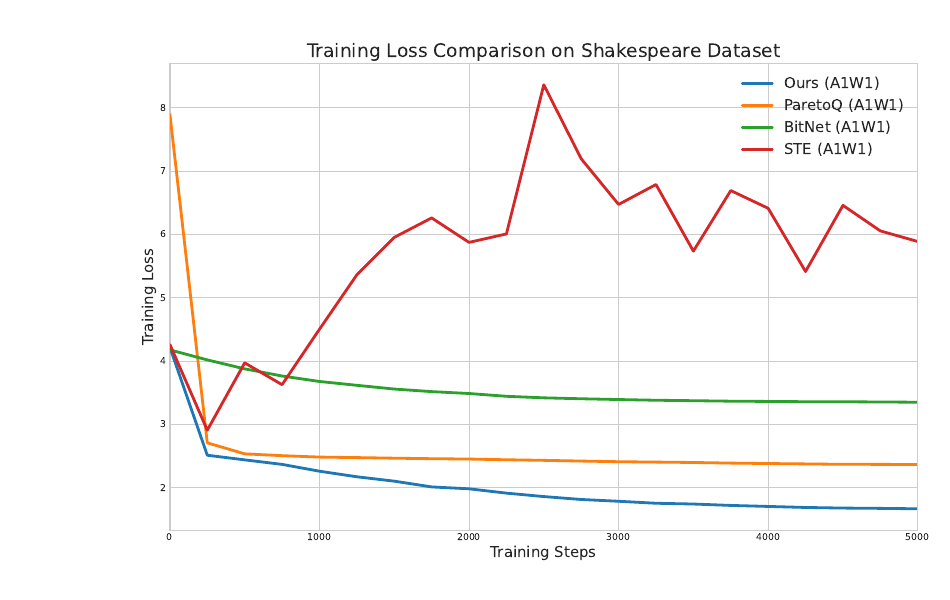
\includegraphics[width=\linewidth]{figs/fig1a_ste_divergence.png}\\[4pt]
\small Training loss, 1-bit weights and activations (A1W1), small GPT on Shakespeare. STE (red) diverges; the paper's method (blue) converges.
\end{shadedblock}
\end{minipage}\hfill
\begin{minipage}[t]{0.49\textwidth}
\begin{shadedblock}[\figheight]\centering
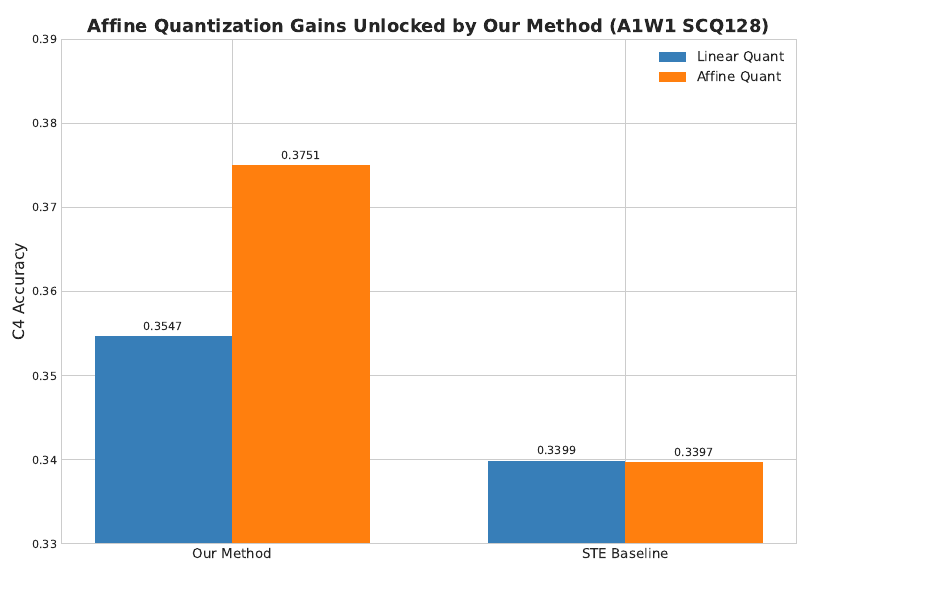
\includegraphics[width=\linewidth]{figs/fig1b_affine.png}\\[4pt]
\small Accuracy at A1W1, linear vs.\ affine quantization. Under STE affine gives no gain; with the paper's method it does.
\end{shadedblock}
\end{minipage}

\vfill
\noindent{\small\textit{Source:} Ye et al., ``Robust Training of Neural Networks at Arbitrary Precision and Sparsity,'' ICLR 2026, Fig.~1.}

\slide{The proposed approach: a denoising reconstruction $g$}

{\setlength{\abovedisplayskip}{4pt}\setlength{\belowdisplayskip}{4pt}
\noindent\textbf{The change.}\quad Keep $f$ and round. Replace $\hat x$ by a fitted reconstruction $g$.
\begin{shadedblock}
\begin{minipage}[t]{0.29\linewidth}\centering
\textbf{Reconstruction.}\par\vspace{4pt}
A new affine map.\par\vspace{14pt}
$\hat x=s_f\,q+b_f\mathbf 1$\par\vspace{5pt}
$\big\downarrow$\par\vspace{5pt}
$g(q)=s_g\,q+b_g\mathbf 1$\par
\end{minipage}\hfill\raisebox{-15mm}{\Large$\Longrightarrow$}\hfill
\begin{minipage}[t]{0.29\linewidth}\centering
\textbf{Ridge regression objective.}\par\vspace{4pt}
Fit $s_g$ and $b_g$ to $x$.\par\vspace{14pt}
$\displaystyle\min_{s_g,\,b_g}\ \frac{1}{2N}\big\|s_g\,q+b_g\mathbf 1-x\big\|^2+\frac{\lambda}{2}\,s_g^2$\par
\end{minipage}\hfill\raisebox{-15mm}{\Large$\Longrightarrow$}\hfill
\begin{minipage}[t]{0.29\linewidth}\centering
\textbf{Solution.}\par\vspace{4pt}
Ridge regression has a closed form.\par\vspace{14pt}
$\displaystyle s_g=\frac{\Cov_{xq}}{\Var_q+\lambda},\qquad b_g=\bar x-s_g\,\bar q$\par\vspace{8pt}
{\itshape $\lambda$ is the regularization parameter.\par}
\end{minipage}
\end{shadedblock}

\vspace{6pt}
\noindent\textbf{Training with $g$.}\quad One forward and one backward pass.
\begin{shadedblock}
\paragraph{Forward pass.} The next layer gets $g(q)$, not $\hat x$.
\[
x\ \xrightarrow{\ f\ }\ f(x)\ \xrightarrow{\ \operatorname{round}\ }\ q\ \xrightarrow{\ g\ }\ g(q)\ \longrightarrow\ \text{rest of network}\ \longrightarrow\ L
\]

\paragraph{Backward pass.} Round stays straight through, as in STE. But $g$ now depends on $\delta$.
\[
\nabla_xL\ \xleftarrow[\text{straight through}]{\ \times\,1/s_f\ }\ \nabla_qL\ \xleftarrow[\text{depends on }\delta]{\ \times\,(\partial g/\partial q)^{\top}\ }\ \nabla_gL\ \longleftarrow\ \text{rest of network}\ \longleftarrow\ L
\]
\end{shadedblock}
}

\slide{Why it works: the backward pass sees $\delta$}

{\setlength{\abovedisplayskip}{2pt}\setlength{\belowdisplayskip}{2pt}
\paragraph{The idea.} Both methods treat round's slope as 1, so $\partial q/\partial x=I/s_f$. Only the step after round differs.

\begin{shadedblock}
\paragraph{STE.} $\hat x=s_f\,q+b_f\mathbf 1$ has the same slope for every $\delta$.
\[
\nabla_xL=\underbrace{\Big(\frac{1}{s_f}\,\frac{\partial \hat x}{\partial q}\Big)^{\!\top}}_{\text{local}\;=\;I}\ \underbrace{\vphantom{\Big(}\nabla_{\hat x}L}_{\text{upstream}}=\nabla_{\hat x}L
\]
\end{shadedblock}

\begin{shadedblock}
\setlength{\abovedisplayskip}{3pt}\setlength{\belowdisplayskip}{3pt}
\paragraph{With $g$.} The gradient reaches $x$ by two paths. Local gradient times upstream gradient:\par\vspace{6pt}
\noindent\begin{minipage}{0.60\linewidth}\centering
$\displaystyle
\nabla_xL=\underbrace{\Big(\underbrace{\frac{1}{s_f}\,\frac{\partial g}{\partial q}}_{\text{through $q$}}\;+\;\underbrace{\vphantom{\frac{1}{s_f}}\frac{\partial g}{\partial x}}_{\text{through $x$}}\Big)^{\!\top}}_{\text{local}}\ \underbrace{\vphantom{\Big(}\nabla_gL}_{\text{upstream}}
$
\end{minipage}\hfill
\begin{minipage}{0.38\linewidth}\centering
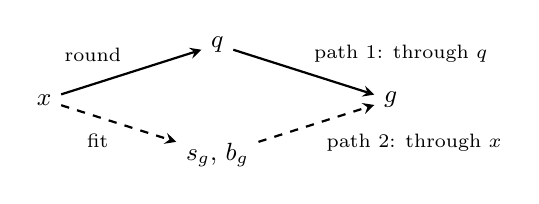
\begin{tikzpicture}[>=stealth,every node/.style={font=\small}]
\node (x) at (0,0) {$x$};
\node (q) at (2.2,0.7) {$q$};
\node (s) at (2.2,-0.7) {$s_g,\,b_g$};
\node (g) at (4.4,0) {$g$};
\draw[->,thick] (x) -- node[above left,font=\scriptsize]{round} (q);
\draw[->,thick] (q) -- node[above right,font=\scriptsize]{path 1: through $q$} (g);
\draw[->,thick,dashed] (x) -- node[below left,font=\scriptsize]{fit} (s);
\draw[->,thick,dashed] (s) -- node[below right,font=\scriptsize]{path 2: through $x$} (g);
\end{tikzpicture}
\end{minipage}\par\vspace{10pt}
\noindent
\begin{minipage}[t]{0.52\linewidth}
\textbf{Through $q$.} Changes with the rounding error. It carries $\delta$ into the gradient:
\[
\frac{\partial g}{\partial q}=\underbrace{\vphantom{\Big(\frac{\partial s_g}{\partial q}\Big)}s_g\,I}_{\mathclap{\substack{\text{like STE's }s_fI\text{,}\\\text{but }s_g\text{ carries }\delta}}}\quad+\;\;\underbrace{q\Big(\frac{\partial s_g}{\partial q}\Big)^{\!\top}+\mathbf 1\Big(\frac{\partial b_g}{\partial q}\Big)^{\!\top}}_{\substack{\text{new terms,}\\\text{carry }\delta\text{ through }x-g(q)}}
\]
\end{minipage}\hfill
\begin{minipage}[t]{0.44\linewidth}
\textbf{Through $x$.} For the current $q$, $g$ is linear in $x$.\par\vspace{8pt}
{\centering\itshape No information about the rounding error.\par}
\end{minipage}
\end{shadedblock}
}


\slide{Results from the paper}

\newcommand{\resheight}{30mm}
\begin{shadedblock}
\paragraph{Gemma 3 language model (1B), trained from scratch.} Score: share of next tokens predicted correctly.\par\vspace{8pt}
\begin{center}
\renewcommand{\arraystretch}{1.3}
\begin{tabular}{lccc}
\toprule
bits for weights and activations & STE & with $g$ & gain \\
\midrule
4 & 0.425 & 0.427 & $+0.002$ \\
2 & 0.379 & 0.403 & $+0.024$ \\
1 & 0.340 & 0.375 & $+0.035$ \\
\bottomrule
\end{tabular}\par\vspace{8pt}
\textit{The fewer the bits, the bigger the gain.}
\end{center}
\end{shadedblock}

\vspace{6pt}
\noindent
\begin{minipage}[t]{0.49\textwidth}
\begin{shadedblock}[\resheight]
\textbf{Extension to sparsity.}\par\vspace{3pt}Pruned and quantized 4B beats full 1B.\par\vspace{4pt}
\begin{itemize}\setlength{\itemsep}{6pt}
\item 4B, 1-bit weights, half pruned: 650 MB, score 0.452.
\item 1B, full precision: 1400 MB, score 0.449.
\end{itemize}
\end{shadedblock}
\end{minipage}\hfill
\begin{minipage}[t]{0.49\textwidth}
\begin{shadedblock}[\resheight]
\textbf{Other domains.}\par\vspace{3pt}At 4 bits, images and translation match full precision.\par\vspace{4pt}
\begin{itemize}\setlength{\itemsep}{6pt}
\item Images (ResNet-50): 76.45\% at 4 bits, 76.41\% full precision.
\item Translation: 29.71 BLEU at 4 bits, 29.49 full precision.
\end{itemize}
\end{shadedblock}
\end{minipage}

\slide{Our implementation 1: the paper's 1-bit GPT}
\noindent\textbf{Setup.}\quad Small GPT on Shakespeare, the paper's exact settings, 1-bit weights and activations.

\begin{shadedblock}
\centering
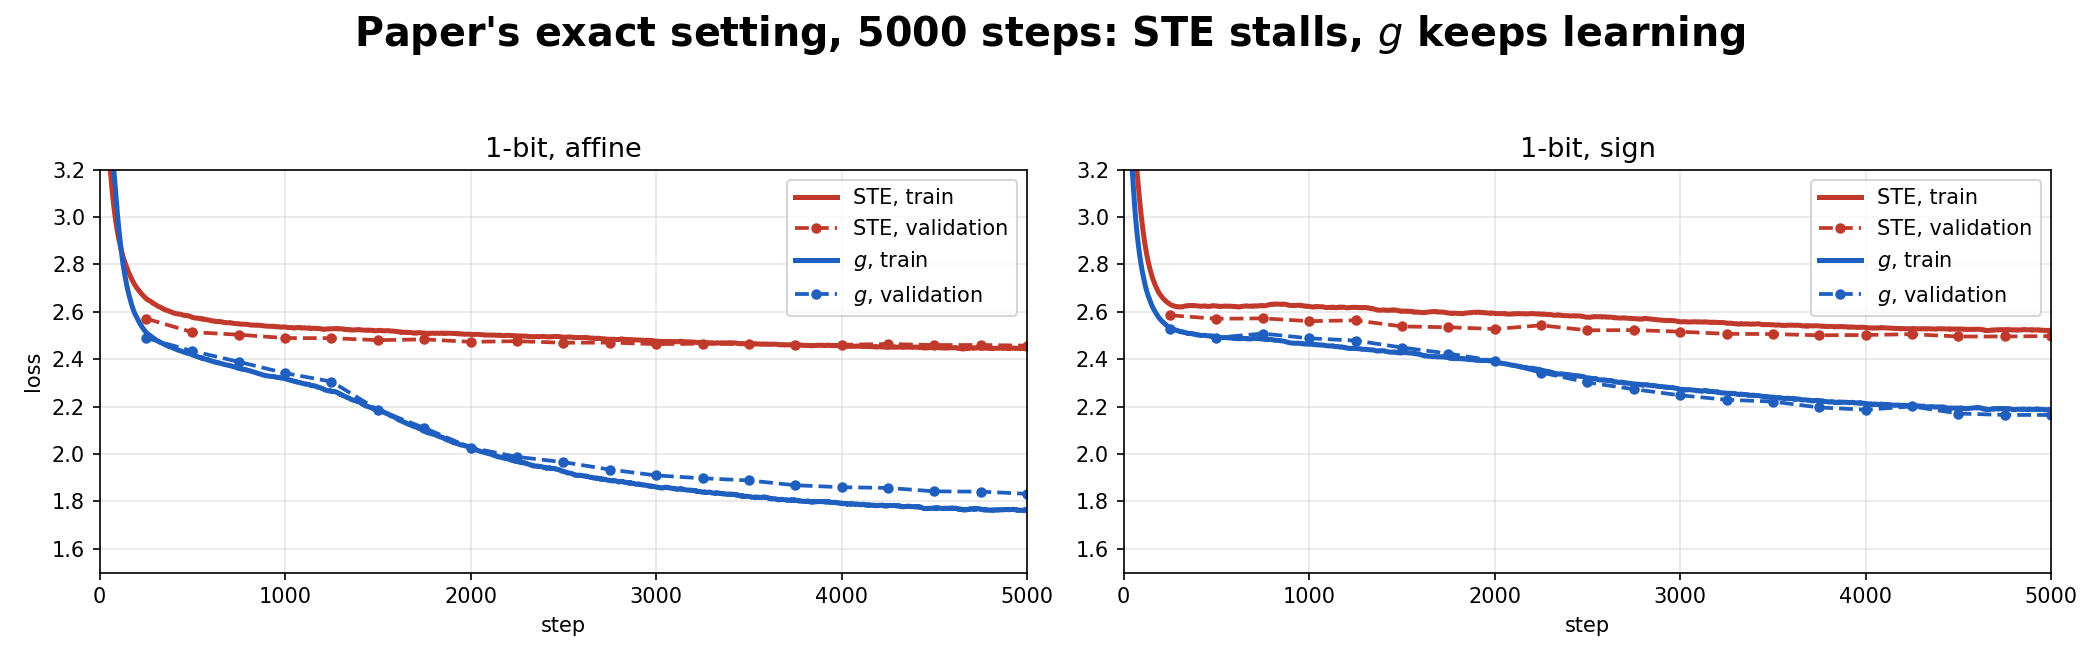
\includegraphics[width=0.86\linewidth]{implementation/onebit/plots/loss_full.png}
\end{shadedblock}

\begin{shadedblock}
\begin{itemize}\setlength{\itemsep}{6pt}
\item \textbf{STE stalls, $g$ keeps learning.} Final loss 2.41 against 1.65.
\item \textbf{$g$ reproduces the paper's curve.} Within 0.05 at every checkpoint.
\item \textbf{STE does not blow up here.} The paper's STE climbs to about 6.
\end{itemize}
\end{shadedblock}

\vfill
\noindent{\footnotesize\textit{Reference:} model and recipe follow nanoGPT by A.~Karpathy, \texttt{github.com/karpathy/nanoGPT}.}

\slide{Our implementation 2: solving a real-world task}
\noindent\textbf{Task.}\quad Label each satellite image as one of 10 land types, such as forest or river.\par\vspace{2pt}
\noindent\textbf{Model.}\quad A small vision transformer (2.7M parameters, 6 layers), quantized to different precisions.
\newcommand{\eurosatheight}{66mm}

\noindent
\begin{minipage}[t]{0.63\textwidth}
\begin{shadedblock}[\eurosatheight]
\vspace*{\fill}\centering
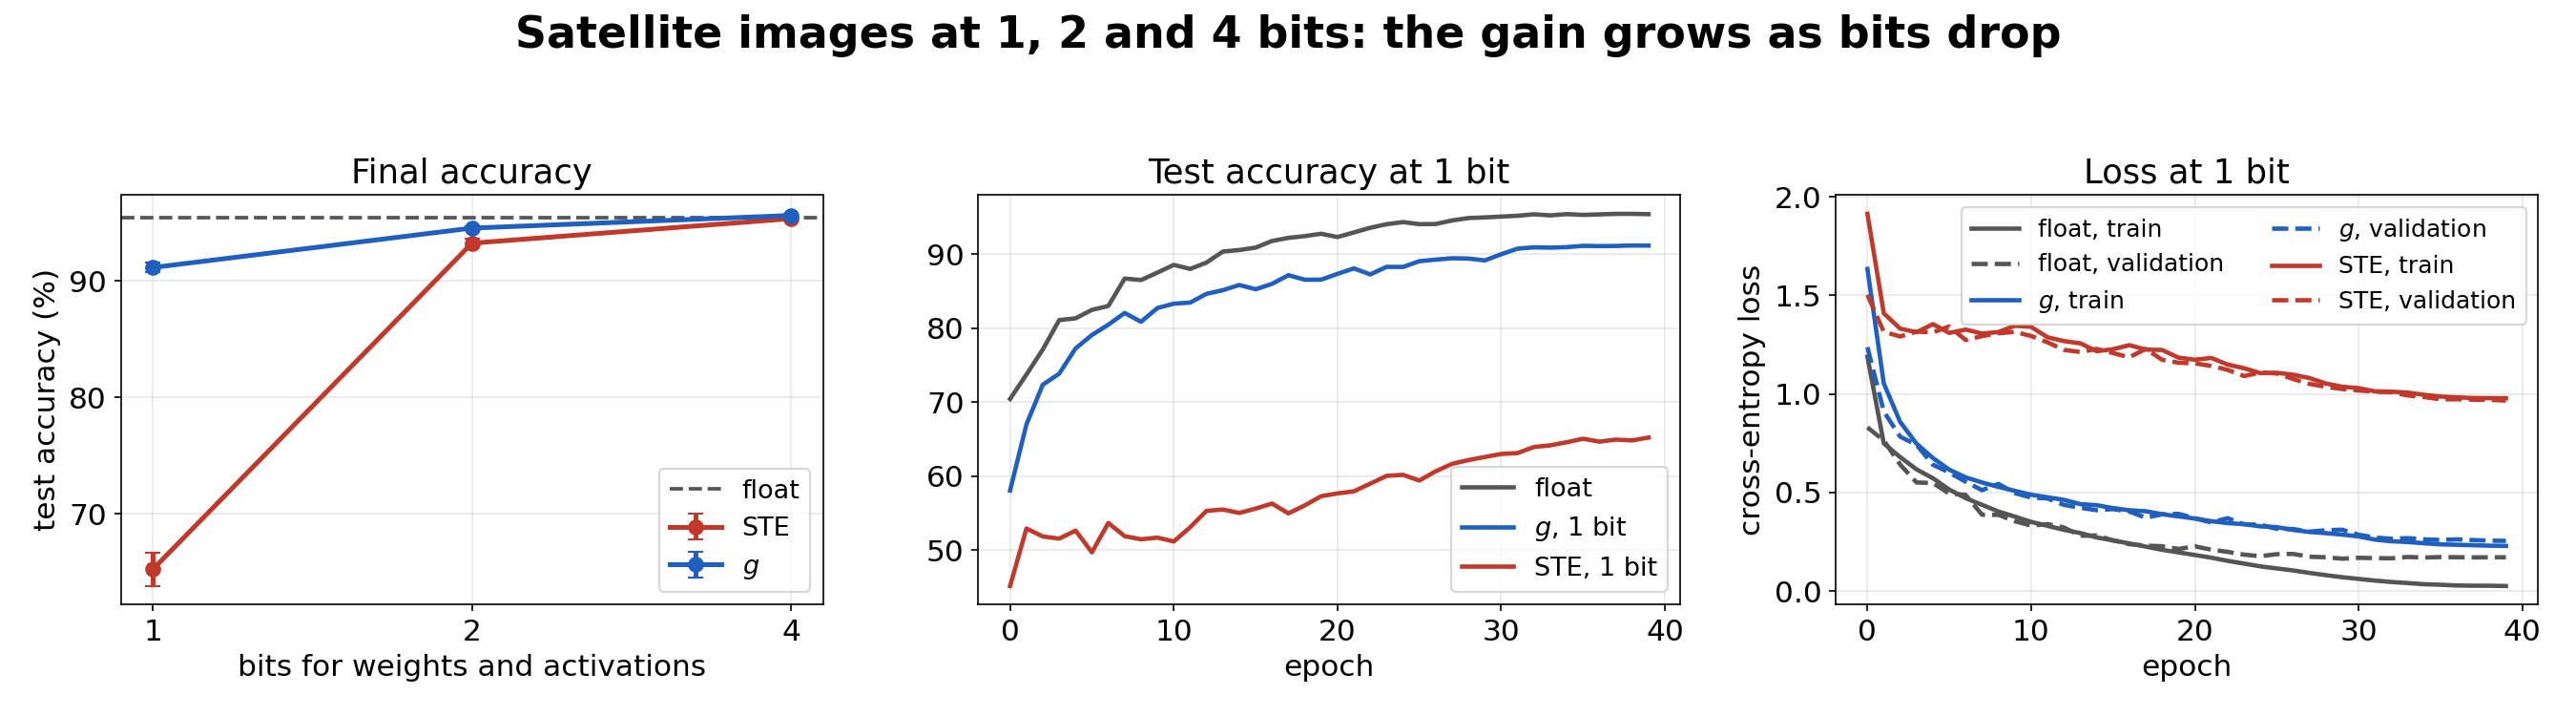
\includegraphics[width=\linewidth]{implementation/vit/plots/eurosat_results.png}
\vspace*{\fill}
\end{shadedblock}
\end{minipage}\hfill
\begin{minipage}[t]{0.355\textwidth}
\begin{shadedblock}[\eurosatheight]
\vspace*{\fill}\centering
\textbf{Test accuracy (\%).}\par\vspace{8pt}
\renewcommand{\arraystretch}{1.2}
\begin{tabular}{lccc}
\toprule
 & 4 bits & 2 bits & 1 bit \\
\midrule
STE & 95.4 & 93.3 & 65.2 \\
with $g$ & 95.6 & 94.5 & \textbf{91.2} \\
\textbf{gain} & $\mathbf{+0.2}$ & $\mathbf{+1.2}$ & $\mathbf{+26.0}$ \\
\bottomrule
\end{tabular}\par\vspace{12pt}
\textit{Full precision: 95.4\%.}\par\vspace{6pt}
\textit{The gain over STE grows as bits drop.}
\vspace*{\fill}
\end{shadedblock}
\end{minipage}

\vfill
\noindent{\footnotesize\textit{Data:} P.~Helber et al., ``EuroSAT: a novel dataset and deep learning benchmark for land use and land cover classification,'' IEEE JSTARS, 2019.}

\slide{Advantages and disadvantages}
\newcommand{\advheight}{78mm}

\vspace{14pt}
\noindent
\begin{minipage}[t]{0.48\textwidth}
\textbf{Advantages.}
\begin{shadedblock}[\advheight]
\vspace{0pt plus 0.6fill}
\begin{itemize}\setlength{\itemsep}{0pt plus 1fill}
\point{Makes 1-bit training work.}{The fitted reconstruction keeps training stable.}
\point{Better reconstruction.}{Closer to $x$ than standard dequantization.}
\point{Extends to sparsity.}{Pruning is one more rounding step, then $g$:\\[4pt]
$x\ \xrightarrow{\ \operatorname{threshold}\ }\ x_S\ \xrightarrow{\ f,\ \operatorname{round}\ }\ q\ \xrightarrow{\ g\ }\ g(q)$}
\end{itemize}
\vspace{0pt plus 0.6fill}
\end{shadedblock}
\end{minipage}\hfill
\begin{minipage}[t]{0.48\textwidth}
\textbf{Disadvantages.}
\begin{shadedblock}[\advheight]
\vspace{0pt plus 0.6fill}
\begin{itemize}\setlength{\itemsep}{0pt plus 1fill}
\point{Round is still straight through.}{``Without gradient estimation'' is too strong.}
\point{Small gain at 4 bits.}{Only $+0.002$, \textit{in the most common setting.}}
\point{Savings are estimates.}{No real hardware, no speed numbers.}
\end{itemize}
\vspace{0pt plus 0.6fill}
\end{shadedblock}
\end{minipage}

\slide{Our takeaways}
\newcommand{\takeheight}{60mm}

\vspace{10pt}
\noindent
\begin{minipage}[t]{0.48\textwidth}
\vspace{0pt}\textbf{What convinced us.}
\begin{shadedblock}[\takeheight]
\begin{itemize}\setlength{\itemsep}{14pt}
\point{A clean comparison.}{Only the reconstruction differs between the two methods.}
\point{Consistent gains.}{$g$ wins in every setting, more at fewer bits.}
\point{Our 1-bit run agrees.}{STE stalls; $g$ keeps learning.}
\end{itemize}
\end{shadedblock}
\end{minipage}\hfill
\begin{minipage}[t]{0.48\textwidth}
\vspace{0pt}\textbf{Open question.}
\begin{shadedblock}[\takeheight]
\vspace*{\fill}
{\centering\textbf{``No gradient estimation''.}\par\vspace{12pt}
The paper claims it (abstract; Table 8).\par\vspace{8pt}
But $\delta$ is detached, exactly as in STE:\par\vspace{10pt}
$q=f(x)+\operatorname{stopgrad}(\delta)\ \Rightarrow\ \partial q/\partial f(x)=I$\par}
\vspace*{\fill}
\end{shadedblock}
\end{minipage}

\vfill
\begin{shadedblock}
{\centering
\textbf{Takeaway}\\[6pt]
A good approximation can still cause optimization issues.\\[4pt]
Rounding error looks ignorable, but training needs its information.\\[4pt]
Fitting parameters to the data is a good bet.\par}
\end{shadedblock}

\end{document}
